%%=============================================================================
%% Resultaten
%%=============================================================================

\chapter{\IfLanguageName{dutch}{Resultaten}{Results}}%
\label{ch:resultaten}


\section{\IfLanguageName{dutch}{Incidenten}{Incidents}}
\label{sec:incidenten-resultaten}

In sectie \ref{sec:evaluatie-criteria} was er sprake over feedback van de werknemers van Evolane.
Aangezien Netskope tijdens de evaluatieperiode al reeds in gebruik was, moest de DLP-oplossing hierop verder bouwen
Tijdens de eerste weken was het initieel het doel om de DLP-regels van \textit{User-Alert} naar \textit{Block} te zetten.
Maar omdat Netskope bij veel werknemers uitstond door een slechte configuratie van voordien, is hier ook geen verdere feedback op gekomen.
Netskope zorgde bijvoorbeeld ervoor dat werknemers niet naar klanten-websites konden surfen, \texttt{dig} werkte niet altijd meer, enzovoort.
Tijdens de momenten dat Netskope wel opstond, waren er een aantal incidenten vastgesteld.
De incidenten gingen dan over klantendocumenten die over Slack en Email werden verstuurd. 
Deze incidenten stelden wel vast dat het \textit{Security} team van Evolane heel andere confidentiële data verwerkt, vergeleken met het \textit{Sales} team.

\begin{figure}[h]
    \centering
    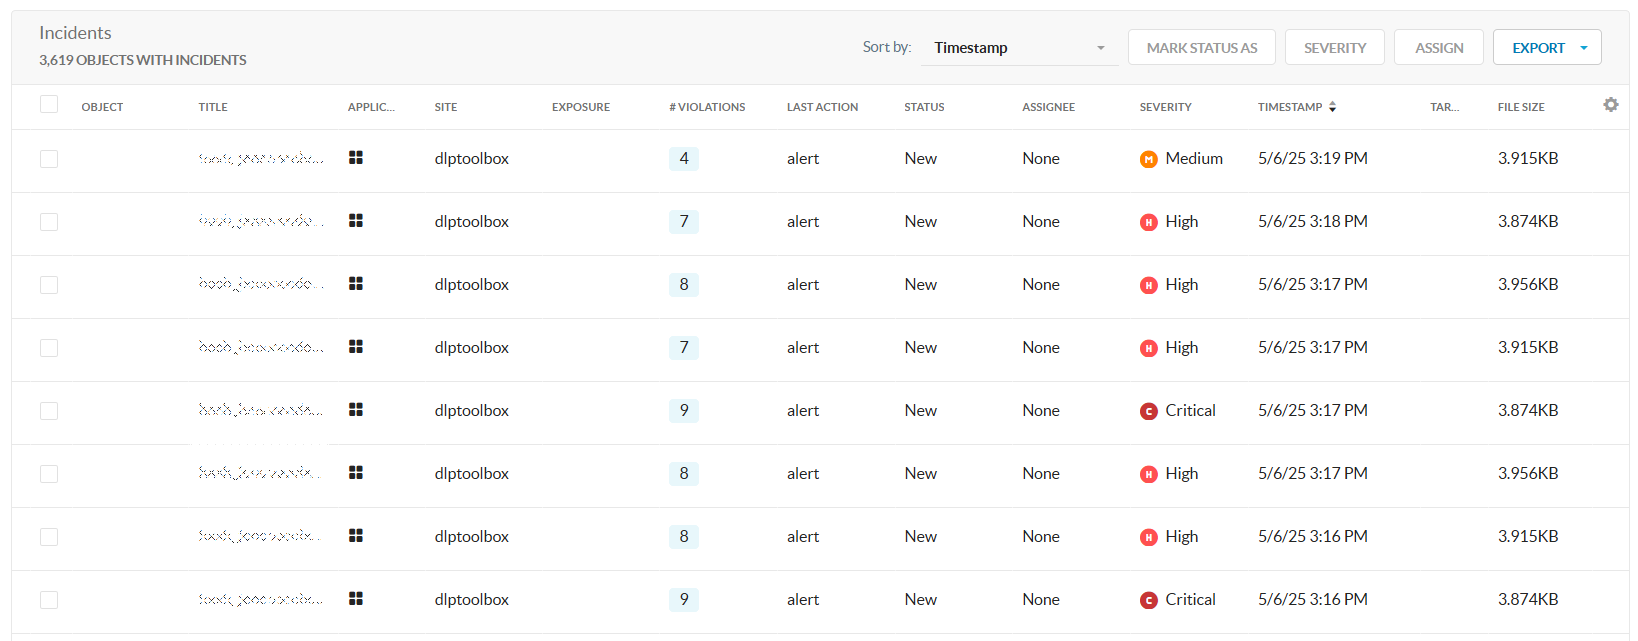
\includegraphics[width=0.8\textwidth]{img/netskope_incidents2.png}
    \caption{Incidenten in Netskope}
    \label{fig:netskope_incidenten}
\end{figure}

\section{\IfLanguageName{dutch}{Vooraf gedefinieerde DLP-regels}{Predefined DLP rules}}
\label{sec:res-vooraf-gedefinieerde-dlp-regels}


\subsection{\IfLanguageName{dutch}{Functionaliteit}{Functionality}}
\label{sec:functionaliteit-resultaten-vooraf}


\subsection{\IfLanguageName{dutch}{Correctheid}{Correctness}}
\label{sec:correctheid-resultaten-vooraf}

Zoals vermeld in Sectie \ref{sec:correctheid} zal de correctheid van de DLP-regels worden geëvalueerd aan de hand van een confusion matrix \ref{tab:confusion_matrix}. 
Tabel \ref{tab:confusion_matrix-vooraf} toont de confusion matrix voor de vooraf gedefinieerde DLP-regels. 
De evaluatieperiode liep van 22 april 2025 tot en met 25 mei 2025. 
In de eerste week werden alle eigen gemaakte regels in een evaluatie modus gezet. 
De eindgebruiker kreeg een melding wanneer er een verwerking van gevoelige data plaatsvond, maar de verwerking werd niet geblokkeerd. 
In dezelfde week en de weken erna werden de regels verder geconfigureerd en getest. 


\begin{table}[h]
    \centering
    \small
    \scriptsize
    \begin{tabular}{|c|c|c|}
        \hline
        \textbf{} & \textbf{Werkelijke Gevoelige Data} & \textbf{Geen Gevoelige Data} \\ \hline
        \textbf{Gedetecteerd als gevoelig} & TP & FP \\ \hline
        \textbf{Niet gedetecteerd als gevoelig} & FN & TN \\ \hline
    \end{tabular}
    \caption{Confusion Matrix voor regex-detectie}
    \label{tab:confusion_matrix-vooraf}
\end{table}


\subsubsection{\iflanguage{dutch}{Hoe eenvoudig is het om de DLP-regels te configureren?}{false}}
\label{}

% Aangezien deze regels vooraf zijn gedefinieerd, kan je dit direct toepassen op de organisatie. 
% Er is bijvoorbeeld geen mogelijkheid om de thresholds te veranderen. 
% Wat lastig kan zijn als je DLP regels wilt toepassen 

1. Niet aanpasbare profielen/regels (Geen mogelijkheid om thresholds te veranderen)
2. Entiteiten zijn niet publiek (moeilijk evalueren als je niet weet wat er mist)

\subsubsection{\iflanguage{dutch}{Is er voldoende documentatie beschikbaar voor de DLP-regels?}{false}}
\label{}

Ja, zoals te merken in dit onderzoek, staat het hier vol mee

\subsubsection{\iflanguage{dutch}{Hoe eenvoudig is het om de DLP-regels te gebruiken?}{false}}
\label{}

Moeilijk met deze

\subsubsection{\iflanguage{dutch}{Is er voldoende ondersteuning beschikbaar voor de DLP-regels?}{false}}
\label{}

Ja, gemakkelijk te clonen om zelf regels aan te maken/ aan te passen

\section{\IfLanguageName{dutch}{Eigen gedefinieerde DLP-regels}{Custom DLP rules}}
\label{sec:res-eigen-gedefinieerde-dlp-regels}


\subsection{\IfLanguageName{dutch}{Functionaliteit}{Functionality}}
\label{sec:functionaliteit-resultaten-eigen}

\subsection{\IfLanguageName{dutch}{Correctheid}{Correctness}}
\label{sec:correctheid-resultaten-eigen}

\textcite{Quaeyhaegens2025}, \textit{Partner Solution Architect} bij \textbf{Netskope}, verklaarde tijdens \textit{Cybersec Europe}: 
``Netskope DLP-incidenten kunnen false positives bevatten, maar genereren nooit false negatives''. 
Deze uitspraak is een persoonlijke notitie. 
DLP-systemen detecteren uitsluitend gegevens die voldoen aan gedefinieerde regels, waardoor relevante matches altijd in beeld komen zolang de configuratie correct blijft.

% Quaeyhaegens2025


\begin{table}[h]
    \centering
    \small
    \scriptsize
    \begin{tabular}{|c|c|c|}
        \hline
        \textbf{} & \textbf{Werkelijke Gevoelige Data} & \textbf{Geen Gevoelige Data} \\ \hline
        \textbf{Gedetecteerd als gevoelig} & TP & FP \\ \hline
        \textbf{Niet gedetecteerd als gevoelig} & FN & TN \\ \hline
    \end{tabular}
    \caption{Confusion Matrix voor regex-detectie}
    \label{tab:confusion_matrix-eigen}
\end{table}

\section{\IfLanguageName{dutch}{Performantie}{Performance}}
\label{sec:performantie-resultaten}

% Om de impact van de Netskope-agent op de netwerkperformantie te evalueren, werd gebruik gemaakt van de tool \texttt{iPerf3}. 
% De tests werden uitgevoerd op een macOS-systeem, met telkens een client-verbinding naar een publieke \texttt{iperf3}-server. 

% Elke test liep gedurende 60 seconden met een logging-interval van 5 seconden. Onderstaande tabel toont de gemiddelde throughput en eventuele merkbare vertraging.
% De testscenario's~\ref{tab:test-scenarios-performance} gaven volgende resultaten:

% Tijdens de test met actieve agent werd ook het netwerkverkeer geanalyseerd via \texttt{Wireshark}. 
% Hieruit blijkt dat de agent actief verbindingen intercept via een lokale proxy (TCP verbinding naar \texttt{127.0.0.1:port}) alvorens verkeer door te sturen. 
% Deze interceptie introduceert merkbare vertraging bij uploads van gevoelige bestanden, wat zichtbaar is in de lagere throughput en hogere latency. 
% % \item Wireshark bevestigde TLS-interceptie bij upload van een testbestand met dummy persoonsgegevens.

%  .\iperf3.exe -s
% ngrok tcp 5201 


% \begin{table}[h]
%     \centering
%     \begin{tabular}{lcc}
%         \toprule
%         \textbf{Testscenario} & \textbf{Gemiddelde download (Mbps)} & \textbf{Retransmissies} \\
%         \midrule
%         Zonder Netskope             & 94.5 & 0 \\
%         Met Netskope (passief)      & 89.2 & 1 \\
%         Met Netskope (DLP actief)   & 74.8 & 3 \\
%         Met Netskope (Tijdens upload) & 65.3 & 5 \\
%         \bottomrule
%     \end{tabular}
%     \caption{Netwerkperformance met en zonder Netskope (gemeten via \texttt{iPerf3})}
%     \label{tab:iperf3-results}
% \end{table}

\section{\IfLanguageName{dutch}{Gebruiksvriendelijkheid}{User-friendliness}}
\label{sec:gebruiksvriendelijkheid-resultaten}

% Top Alternatieven voor Netskope DLP
% https://www.nightfall.ai/blog/netskope-dlp-comprehensive-analysis-and-top-alternatives

% The Netskope client uses the same method to inspect and filter traffic that the GlobalProtect App uses to implement domain and application-based split tunneling. The Netskope client can prevent traffic from being sent out the correct interface (VPN virtual interface or physical interface).
% https://knowledgebase.paloaltonetworks.com/KCSArticleDetail?id=kA14u0000001VGGCA2&lang=en_US%E2%80%A9#:~:text=The%20Netskope%20client%20uses%20the,virtual%20interface%20or%20physical%20interface



\begin{table}[h]
    \centering
    \small
    \scriptsize
    \begin{tabular}{ll}
        \toprule
        \textbf{Categorie} & \textbf{Waarde / Beschrijving} \\
        \midrule
        \multicolumn{2}{l}{\textbf{Overzicht incidenten}} \\
        Totaal aantal incidenten & 15.088 \\
        Totaal gelogde berichten & 64.000 \\
        Gemiddelde incidenten per bericht & $\approx$ 0,24 \\[4pt]

        \multicolumn{2}{l}{\textbf{Aantal DLP-regels per incident}} \\
        1 regel & 8.921 incidenten \\
        2 regels & 4.439 incidenten \\
        3 regels & 1.342 incidenten \\
        4 regels & 267 incidenten \\
        5 regels & 64 incidenten \\
        6 regels & 29 incidenten \\
        7 regels & 13 incidenten \\
        8 regels & 7 incidenten \\
        9 regels & 1 incident \\
        10 regels & 3 incidenten \\
        19 regels & 1 incident \\
        21 regels & 1 incident \\[4pt]

        \multicolumn{2}{l}{\textbf{Meest getroffen DLP-regels (top 10)}} \\
        EU-Name-email (narrow) & 11.004 keer \\
        EU-Name-Phone (narrow) & 5.423 keer \\
        Name-Email & 3.926 keer \\
        EU-Name-Address (narrow) & 841 keer \\
        EU-Name-Ethnicity (narrow) & 372 keer \\
        EU-Name-Religion (narrow) & 319 keer \\
        Source Code (All) & 236 keer \\
        Name-Medical Condition & 227 keer \\
        EU-Name-Criminal record (narrow) & 203 keer \\
        EU-Name-Political (narrow) & 176 keer \\
        \bottomrule
    \end{tabular}
    \caption{Overzicht van Netskope DLP-incidenten en regelhits}
    \label{tab:netskope_dlp_resultaten}
\end{table}
